\documentclass{article}
\usepackage{fullpage}
\usepackage{graphicx}
\usepackage{wrapfig}
\usepackage{listings}
\usepackage{color}
\usepackage{comment}

\definecolor{mygreen}{rgb}{0,0.6,0}
\definecolor{mygray}{rgb}{0.5,0.5,0.5}
\definecolor{mymauve}{rgb}{0.58,0,0.82}

\lstset{ %
  backgroundcolor=\color{white},   % choose the background color; you must add \usepackage{color} or \usepackage{xcolor}
  basicstyle=\footnotesize,        % the size of the fonts that are used for the code
  breakatwhitespace=false,         % sets if automatic breaks should only happen at whitespace
  breaklines=true,                 % sets automatic line breaking
  captionpos=b,                    % sets the caption-position to bottom
  commentstyle=\color{mygreen},    % comment style
  deletekeywords={...},            % if you want to delete keywords from the given language
  escapeinside={\%*}{*)},          % if you want to add LaTeX within your code
  extendedchars=true,              % lets you use non-ASCII characters; for 8-bits encodings only, does not work with UTF-8
  frame=single,                    % adds a frame around the code
  keepspaces=true,                 % keeps spaces in text, useful for keeping indentation of code (possibly needs columns=flexible)
  keywordstyle=\color{blue},       % keyword style
  language=Octave,                 % the language of the code
  morekeywords={*,...},            % if you want to add more keywords to the set
  numbers=left,                    % where to put the line-numbers; possible values are (none, left, right)
  numbersep=5pt,                   % how far the line-numbers are from the code
  numberstyle=\tiny\color{mygray}, % the style that is used for the line-numbers
  rulecolor=\color{black},         % if not set, the frame-color may be changed on line-breaks within not-black text (e.g. comments (green here))
  showspaces=false,                % show spaces everywhere adding particular underscores; it overrides 'showstringspaces'
  showstringspaces=false,          % underline spaces within strings only
  showtabs=false,                  % show tabs within strings adding particular underscores
  stepnumber=2,                    % the step between two line-numbers. If it's 1, each line will be numbered
  stringstyle=\color{mymauve},     % string literal style
  tabsize=2,                       % sets default tabsize to 2 spaces
  title=\lstname                   % show the filename of files included with \lstinputlisting; also try caption instead of title
}

\title{Heterogeneous Medical Image Computing Framework}

\date{}

\begin{document}
\maketitle

\section{Purpose}

The main purpose of this framework is to:
\begin{itemize}
    \itemsep 1pt
    \item make the parallel processing and visualization of medical images on heterogeneous systems (CPU+GPU) easier.
    \item provide a platform for benchmarking these operations.
\end{itemize}

\section{Features}

The framework should provide features such as:
\begin{enumerate}
    \itemsep 1pt
    \item concurrent visualization of images and volumes (surface, volume and slice rendering).
    \item import and export of data using commonly used formats such as metaimage, raw, itk and vtk.
    \item concurrent streaming of data.
    \item easy interface for processing image data on different devices. 
    \item mechanisms that will ensure that the image data is updated on all devices after it has been altered on one device.
    \item a set of commonly used algorithms.
    \item an easy interface for measuring the runtime of all operations.
    \item an easy way to set up benchmarking of a set of operations and data.
    \item mechanisms for keeping tracking of which data is stored where and how much memory is used to store these data.
\end{enumerate}

\section{Design}

The framework will consist of six main layers as illustrated with colors in figure \ref{fig:diagram}.
The first bottom layer consist of the actual hardware, i.e. the CPUs and GPUs with all of its memory.
The second layer consist of drivers for this hardware and are provided by the hardware manufacturers.
Next is the library layer in turquoise which consist of several libraries that are needed in the framework.
The libraries in this layer consist of:
\begin{itemize}
    \itemsep 1pt
    \item \textbf{OpenCL} - Enables parallel programming of heterogeneous systems
    \item \textbf{OpenGL} - Enables cross-platform visualization
    \item \textbf{OpenCL Utility Library} - Ease the use of OpenCL
    \item \textbf{GLU} - Ease the use of OpenGL
    \item \textbf{GLEW} - Ease the use of OpenGL
    \item \textbf{Qt} - Cross-platform GUI for visualization
\end{itemize}

\begin{figure}[h]
    \centering
    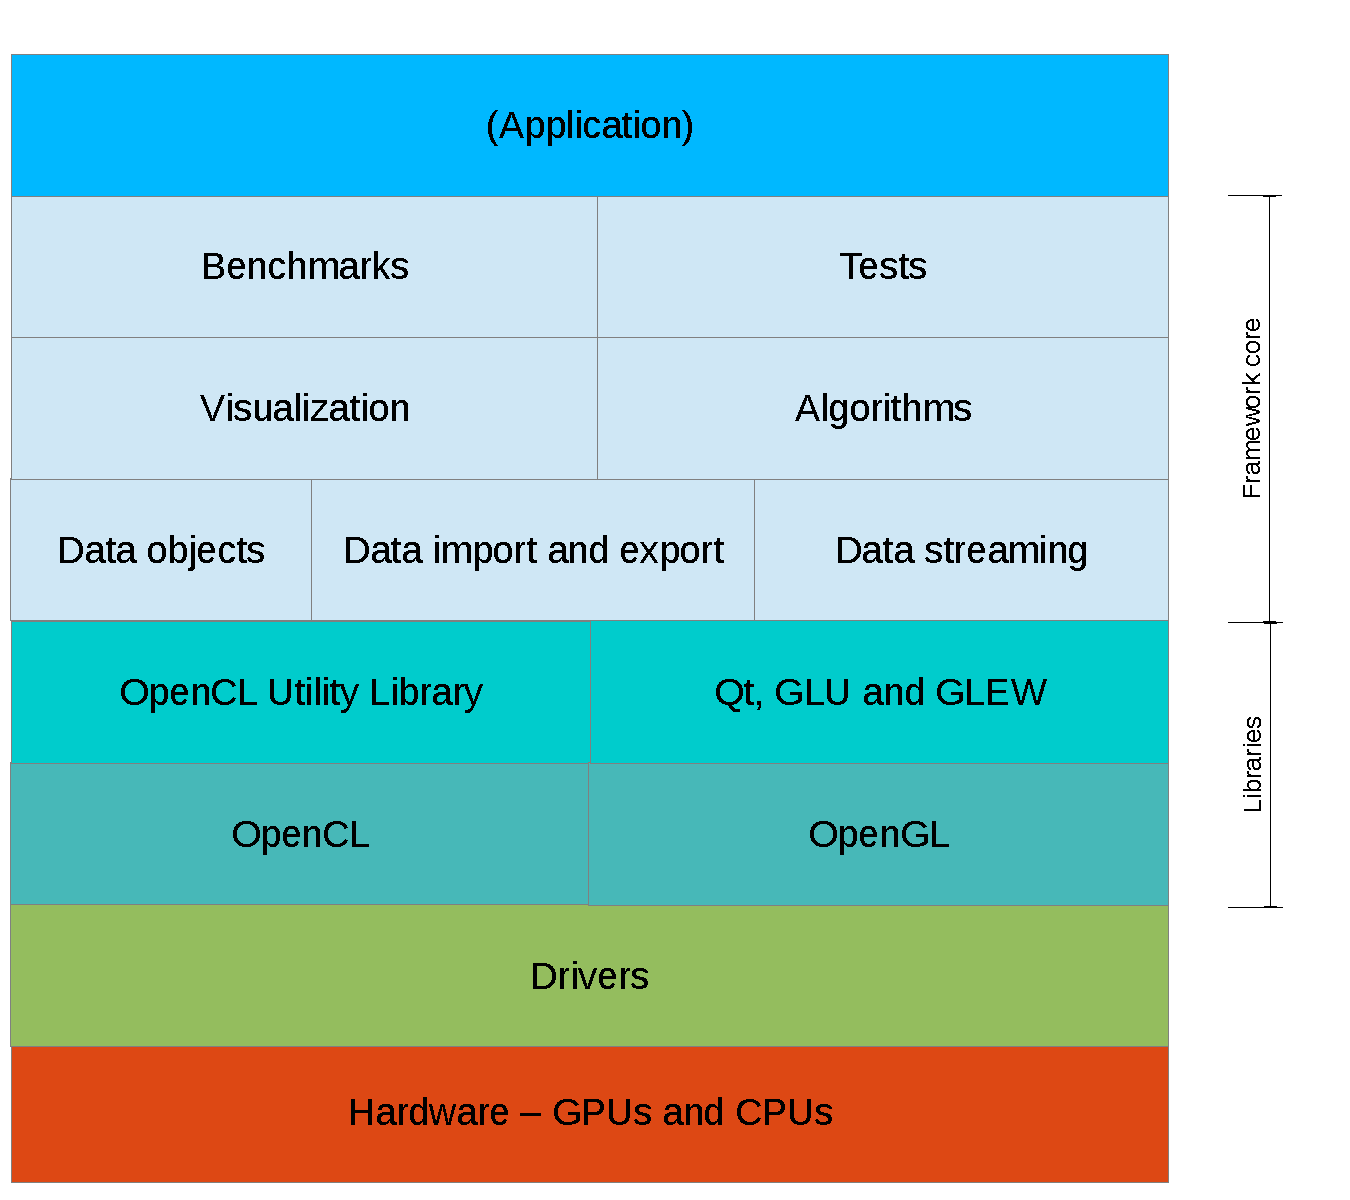
\includegraphics[width=0.75\textwidth]{framework_diagram.pdf}
    \caption{The main layers of the framework.}
    \label{fig:diagram}
\end{figure}

Next is the core of the framework which enables all of the described features in the previous section.
The framework is split into several groups:
\begin{itemize}
    \itemsep 1pt
    \item \textbf{Data objects} - Abstract objects for images, volumes and tracking data which enables the synchronized processing of these data on a set of heterogeneous devices.
    \item \textbf{Data import and export} - Data import and export adapters for different formats such as metaimage, raw, itk and vtk.
    \item \textbf{Data streaming} - Objects that implement Producer/consumer consumer model.
    \item \textbf{Algorithms} - A set of commonly used algorithms.
    \item \textbf{Visualization} - A set of renderers such as surface, volume and slice renderers.
    \item \textbf{Benchmarks} - Mechanisms for measuring, assimilating and reporting the runtime of all operations in the framework.
    \item \textbf{Tests} - A set of tests for the framework which ensures that all parts of the framework are working properly.
\end{itemize}

Finally, on top is the application.
The framework may be both a 1) stand-alone application which enables benchmarking and tests of a heterogeneous system and 2) an external library/framework for another medical image computing application.

\begin{figure}[h]
    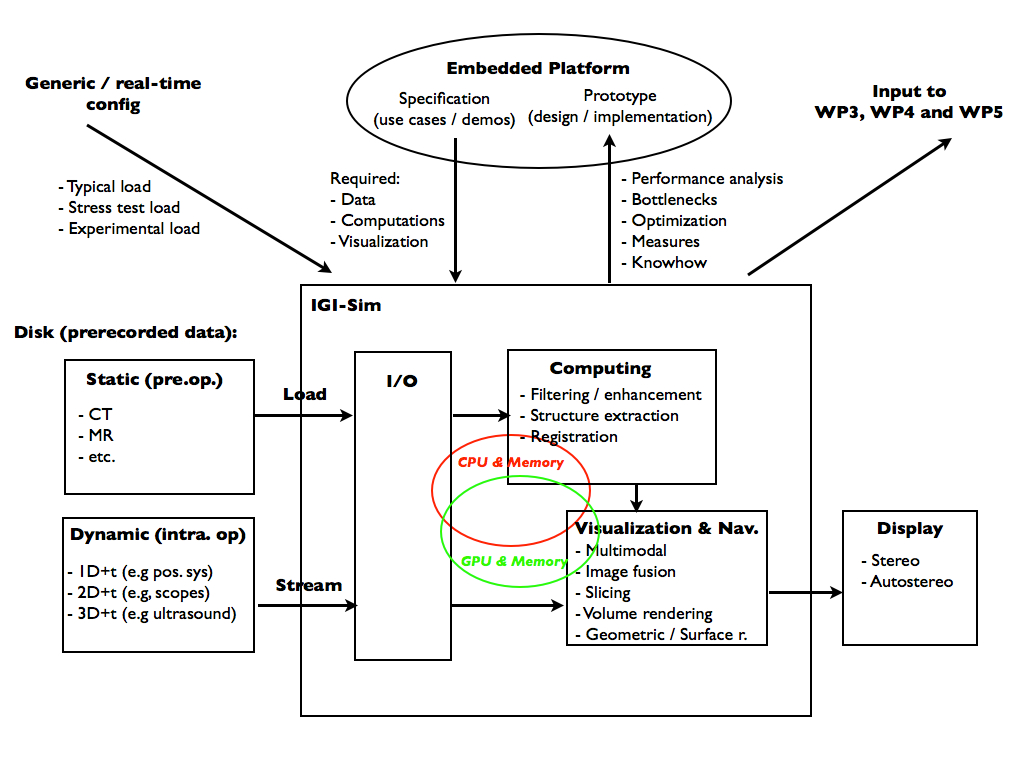
\includegraphics[width=\textwidth]{system_diagram.png}
    \caption{The system}
\end{figure}


\subsection{The execution pipeline}

\begin{figure}
    \centering
    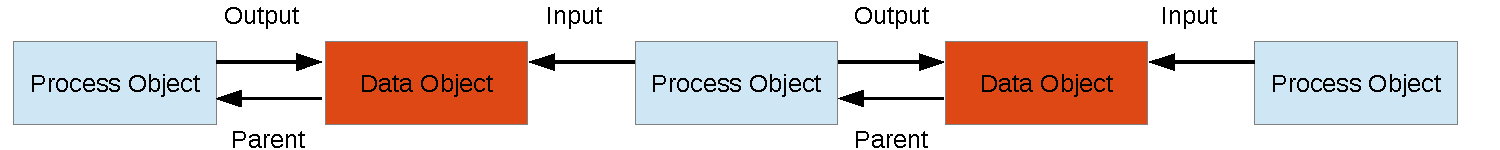
\includegraphics[width=\textwidth]{pipeline_diagram.pdf}
    \caption{A simple pipeline showing how the process and data objects are connected. All the links in this figure are implemented as pointers.}
    \label{fig:pipeline_diagram}
\end{figure}

Data import/export, processing and visualization will are preformed in a demand-driven execution pipeline as in the VTK framework.
The objects that are part of the pipeline are divided into two different groups: data objects and process objects.
Process objects can have multiple input and output data objects while data objects only have a pointer to its parent object that the data object was created from.

After the pipeline has been set up the execution is started by an object requesting up-to-date data by calling update().
When update is called on a pipeline object each object will call update on its parent objects.
When a process object has finished calling update on all its parent objects it will see if any of the parent data objects have changed or if the process object itself has changed (e.g. parameter change) and if so, call the execute() method.
The execute method will perform the actual work and all process objects have to implement this method.

Also, the process objects will have a variable indicating where the object will be executed (OpenCL device, host etc.).


\subsection{Organization of data on heterogeneous devices}

\begin{figure}
    \centering
    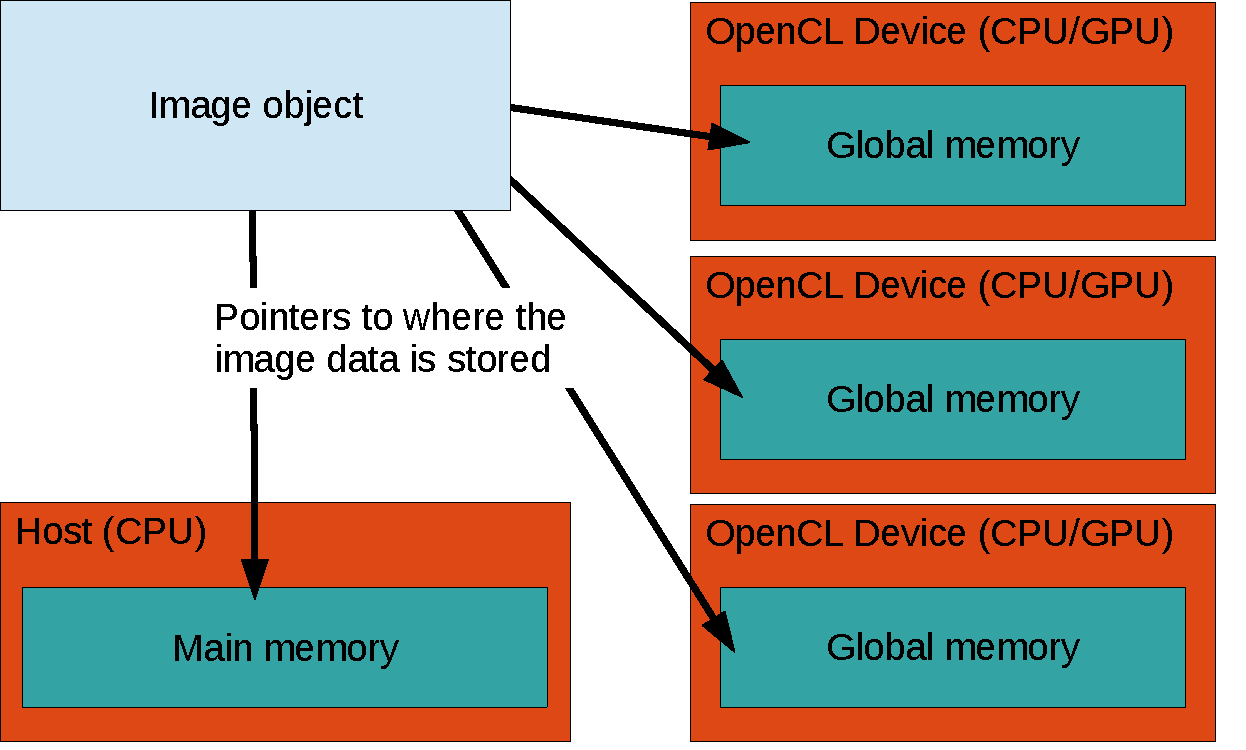
\includegraphics[width=0.55\textwidth]{data_diagram.pdf}
    \caption{Each image object has a set of pointers to where its data is stored. 
        Note that the host is the CPU where the framework is running and may also be an OpenCL device. 
    Also, the image data does not have to be stored in all places, only where it is used.}
    \label{fig:data_diagram}
\end{figure}

Data organization and synchronization is one of the key components in this framework as everything will be built on top of it. 

First off, image data is represented as one of two data objects: \textit{Image2D} or \textit{Image3D}.
These objects represents an image or volume on all devices and its data is guaranteed to be coherent on any device after being altered.
Thus these objects have pointers to all devices where the image data is stored as shown in Figure~\ref{fig:data_diagram}.
If the user wants to change the image while keeping the original image, a copy has to be made.
An image data object has methods for retrieving and manipulating pixels/voxels that are stored on the host (i.e. in the main memory).
The objects also has methods for getting access to the image data on other devices.
The host is the CPU where the framework is executed from.
The host can also be an OpenCL device.
Thus, this framework allows processing of data on the host, using regular C++, and on accelerators such as multi-core CPUs and GPUs using OpenCL.
In this section, it is explained in detail how this is accomplished.

\subsubsection{Data import and export}

Data can be imported and exported to and from the framework in several different forms such as:
\begin{itemize}
    \itemsep 1pt
    \item files on the disk stored in different formats (e.g. metaimage and raw)
    \item memory
    \item OpenCL memory objects
    \item OpenGL memory objects
    \item itk and vtk objects
\end{itemize}
A separate data import and export object exists for each of these types and are used in the constructor of the image objects.
Image data can also be created as an empty image with a specified size and type.

\subsubsection{Images of different data types}

Medical images are represented in different formats.
Some common examples are: Ultrasound (unsigned 8 bit integer), CT (signed/unsigned 16 bit integer) and MR (unsigned 16 bit integer).
And in image processing, several other formats such as 32 and 64 bit floating points numbers and vector types are often used.

The framework will provide the following data formats for images:
\begin{itemize}
    \itemsep 1pt
    \item Signed/unsigned 8 bit integer (char) - CL\_\{UN\}SIGNED\_INT8
    \item Signed/unsigned 16 bit integer (short) - CL\_\{UN\}SIGNED\_INT16
    \item 32 bit floating point number (float) - CL\_FLOAT
    \item 64 bit floating point number (double). (However, not all GPUs support this). - CL\_DOUBLE
    \item Signed/unsigned normalized (-1 to 1 or 0 to 1) 16 bit integer. (Not all GPUs support this) - CL\_\{S\}NORM\_INT16 - This type might just be a modifier of the float type.
    \item Vector types of all above with 2, 3 and 4 components. 
\end{itemize}

To support all of these different data formats without exposing the user to templating the image objects will contain a variable indicating which data type and how many components it has (1-4) and data stored in main memory on the CPU/host will be a void pointer which will be cast to the appropriate type when needed for processing as done in the VTK library.

\subsubsection{Data access}

Two forms of data access are possible in the framework: 1) Read-only, 2) Read and write.
The general rule is that several devices can perform read-only operations on an image coherently.
However, if any device needs to write to an image, only that device can have access to the image at that time.
This is to ensure data coherency across devices.
Thus, if a device wants to write to an image, it has to wait for all other operations on that image to finish.
And when it is writing to the image, no other devices can read or write to that image.

To facilitate this, \textit{DataAccess} objects are introduced.
These objects are created by calling \textit{getAccess} method on the image object.
Arguments to this method are which device wants to access the image and what type of access is desired (Read-only or Read-and-write).
From these objects an OpenCL Image (texture on a GPU) or Buffer object can retrieved which is needed to perform OpenCL computations on the image or pointer to main memory can be request for doing processing on the CPU using C++.
The DataAccess objects also have methods for releasing the access, thus enabling other devices to perform write operations on the image.
The access will also be released in the destructor of this object to avoid programmers creating a deadlock.
When the access is released, the OpenCL Image/Buffer object pointer is invalidated to ensure that the program can no longer manipulate the data.
However, this does not delete the actual data on the device.
When access to an object is requested, the framework should check that any previous access objects have been released.
If not an exception should be thrown.
This is ensure that the user doesn't have multiple access to one image object at the same time.

\subsubsection{Data change}

Every time an image is changed on a device, the change should be reflected on the other devices as well.
However, this doesn't have to be done immediately after the change is finished.
The updating of data can be done the next time the data is requested on another device.
This is often referred to as \textit{lazy loading} in computer science.
The benefit of lazy loading is that the number of data transfers can be reduced.
However, the drawback is that there will be a transfer cost the next time some processing has to be performed on another device which doesn't have the updated data.

Thus, each image object has a set of flags indicating whether the data is not up to date for each device.
When one device has changed some data, these are set to true for all devices except the device in which the change was performed.
Next time the data is requested on a device, the flag is checked and if is true a data transfer will start and the flag will be set to false for that device.

% TODO what about the host

\subsubsection{Data removal}

Memory is limited and it should be possible to delete image data on a specific device explicitly at any location in the code.

% TODO host

\subsubsection{Memory usage}

When data is created and removed it should registered in a MemoryManager singleton object.
This singleton object can be accessed all over the program and be queried for how much memory is used and free on each device.
Should also be possible to register temporary image data in this manager as well.
However, this gives the programmer some responsibility to actually do this to ensure that the memory used/available on a device is correct.
The removal, on the other hand, can be done automatically using the setDestructorCallback method.




\subsection{Concurrent data streaming}

Data streaming is enabled through an implementation of the producer-consumer model.
In this model, there are producers which create/import data and transfers that data to the specified device.
The device will have a limited memory and thus the producer will only fill data in a buffer up to a certain size.
When the buffer is full, the producer will wait until the consumer(s) have finished with that data and then start to fill up the buffer again.

To enable concurrency of the streaming, each data producer runs in a separate thread.
The consumers on the other hand runs in the main thread.
Mutexes and condition variables are used to synchronize the producers and consumers.
For most of the streamers we will only be interested in the newest data and thus a buffer of size 2 images will be sufficient (double buffering).

Different types of streamers should be available in the framework.
E.g. streamers that read data from disk and streamers that receive data from an external source such as an ultrasound scanner.

\subsection{Concurrent visualization}

To allow multiple concurrent visualizations, all rendering and GUI event handling (e.g. keyboard and mouse events) are performed in a separate thread.
This allows visualization of multiple data to be performed while processing from the main thread continues.
The Qt framework is chosen as the graphical user interface (GUI) because:

\begin{itemize}
    \itemsep 1pt
    \item Popular C++ framework, also in the medical domain.
    \item Cross-platform. Supports Windows, Linux and Mac.
    \item Supports multi-threading. (However, the Qt main/event loop is limited to be run in the main thread)
    \item Allows creating windows/widgets that can be rendered to directly by OpenGL.
    \item Supports event handling (keyboard and mouse).
    \item Enables creation of simple forms and buttons.
    \item Object oriented (C++).
\end{itemize}

Four different types of renderers should be available in the framework (the first three are for volumes, while the last one is for images):
\begin{itemize}
    \itemsep 1pt
    \item \textbf{Surface renderer} - Extracts a surface from a volume using the marching cubes algorithm and a threshold parameter. The surface is a triangle mesh which is displayed with OpenGL.
    \item \textbf{Slice renderer} - Extracts data from a volume in an arbitrary plane using trilinear interpolation.
    \item \textbf{Volume renderer} - Creates an image of a volume using ray casting.
    \item \textbf{Image renderer} - For displaying 2D images.
\end{itemize}

A set of renderers can be assigned to a view and a window can exist of several views.

\subsection{Algorithms or "Processing objects"}

An interface for algorithms should be created to ensure that the algorithms are used in coherent way.

All input that doesn't have any default values have to be supplied to the constructor.
Usually, this is just the image to perform the processing on.
Any parameters can be set using setter methods on the processing object.
The output is retrieved through one or several getOutput methods.


\subsection{Tests}

As much as possible of the framework should be covered by unit and system tests to ensure that the framework works properly.
The Catch testing framework is used to create the tests.

\subsection{Benchmarks}

In the future, a scripting language (for instance xml) could be used to create benchmarks.
These could also serve as system tests.

\subsection{Using the framework in a larger application}

The framework may be included and used as part of a larger application for instance through integration with VTK or Qt widgets.

\begin{figure}
    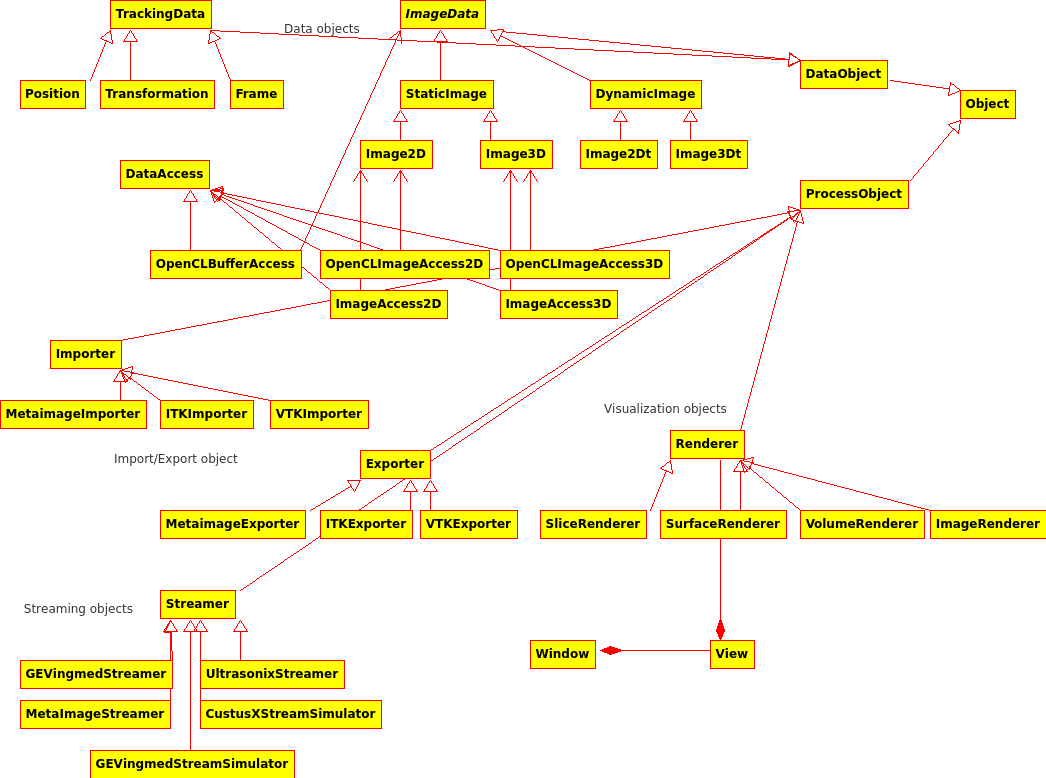
\includegraphics[width=\textwidth]{class_diagram.png}
    \caption{Class diagram}
\end{figure}

\section{Usage examples}

\subsection{Open an image, do some processing and show it on screen}
\begin{lstlisting}[language=C++]
MetaImageImporter::pointer importer = MetaImageImporter::New();
importer->setFilename("filename.mhd");
GaussianSmoothingFilter::pointer filter = GaussianSmoothingFilter::New();
filter->setInput(importer->getOutput());
VolumeRenderer::pointer renderer = VolumeRenderer::New();
renderer->setInput(filter->getOutput());
SimpleWindow::pointer window = SimpleWindow::New(); // A window with only one view
window->addRenderer(renderer);
window->runMainLoop();
\end{lstlisting}

\subsection{Stream images to a device, process and show on screen}
\begin{lstlisting}[language=C++]
MetaImageStreamer::pointer streamer = MetaImageStreamer::New();
streamer->setFilenameFormat("path/filename_#.mhd");
GaussianSmoothingFilter::pointer filter = GaussianSmoothingFilter::New();
filter->setInput(importer->getOutput());
VolumeRenderer::pointer renderer = VolumeRenderer::New();
renderer->setInput(filter->getOutput());
SimpleWindow::pointer window = SimpleWindow::New(); // A window with only one view
window->addRenderer(renderer);
window->runMainLoop();
\end{lstlisting}

\begin{comment}

\subsection{Implementation of a filter}

\begin{lstlisting}[language=C++]
class FilterExample {
    ...
};


void FilterExample::execute() {
    % TODO: implement
    % The filter has to have some identifier to where it is to be executed
    if(this->executeOnHost) {
        this->executeOnHost();
    } else {
        this->executeOnOpenCLDevice(executionDevice);
    }
}

void FilterExample::executeOnOpenCLDevice(oul::Context context) {
    OpenCLImage3DAccess inputAccess = inputImage.getOpenCLImage3DAccess(context, ACCESS_READ);
    cl::Image3D clImage = inputAccess.get();
    OpenCLImage3DAccess outputAccess = outputImage.getOpenCLImage3DAccess(context, ACCESS_READ_WRITE);
    cl::Image3D clOutputImage = outputAccess.get();

    // Do OpenCL processing on clImage using a command queue from context
}

/* These methods are used for serial processing on the host. fancyVTKMacro is used to support different data types without exposing the user to templating */
template <class IT>
void FilterExample::executeOnHost2(IT * input) {
    Image3DAccess outputAccess = outputImage.getPointerAccess(ACCESS_READ_WRITE);
    void * output = outputAccess.get();
    switch(outputImage.getDataType()) {
        fancyVTKMacro(serialAlgorithm(input, (TYPE *)output));
    }
}

void FilterExample::executeOnHost() {
    Image3DAccess inputAccess = inputImage.getPointerAccess(ACCESS_READ);
    void * input = inputAccess.get();
    switch(inputImage.getDataType()) {
        fancyVTKMacro(executeOnHost2((TYPE *)input));
    };
}

template <class IT, class OT> // IT: input type and OT: output type
void FilterExample::serialAlgorithm(IT * input, OT * output) {
    // Do serial processing on the host
}
\end{lstlisting}


\end{comment}

\end{document}
